%=============================================================================
% SECTION 3: MATHEMATICAL WELL-POSEDNESS
% DFD Unified Review --- Part I: Foundations
%=============================================================================

\section{Mathematical Well-Posedness}\label{sec:wellposed}

A physical theory must be mathematically well-posed: given initial/boundary 
data, solutions must exist, be unique, and depend continuously on the data. 
This section establishes these properties for the \DFD field equations in 
both static and dynamic settings.

%-----------------------------------------------------------------------------
% §3.1 STATIC/ELLIPTIC CASE
%-----------------------------------------------------------------------------
\subsection{Static Solutions: Elliptic Theory}\label{sec:elliptic}

\subsubsection{Assumptions on $\mufunction$}

The field equation~\eqref{eq:field_general} is a quasilinear elliptic PDE. 
Well-posedness requires the following conditions on the response function 
$\mufunction: [0,\infty) \to (0,\infty)$:

\begin{itemize}
\item[\textbf{(A1)}] \textbf{Continuity:} $\mufunction$ is continuous on $[0,\infty)$.

\item[\textbf{(A2)}] \textbf{Coercivity:} There exist constants $\alpha > 0$ 
and $p \geq 2$ such that
\begin{equation}
\mufunction(|\xi|)|\xi|^2 \geq \alpha|\xi|^p \quad \forall\,\xi \in \mathbb{R}^3.
\end{equation}
This ensures the energy functional is bounded below.

\item[\textbf{(A3)}] \textbf{Growth bound:} There exists $\beta > 0$ such that
\begin{equation}
|\mufunction(|\xi|)\xi| \leq \beta(1 + |\xi|)^{p-1}.
\end{equation}
This controls the operator's growth at large gradients.

\item[\textbf{(A4)}] \textbf{Monotonicity:} For all $\xi, \eta \in \mathbb{R}^3$,
\begin{equation}
\big(\mufunction(|\xi|)\xi - \mufunction(|\eta|)\eta\big) \cdot (\xi - \eta) \geq 0.
\end{equation}
Strict inequality (strict monotonicity) implies uniqueness.
\end{itemize}

\paragraph{Physical interpretation.}
Condition (A1) ensures continuous transition between regimes. 
Condition (A2) prevents the field from ``running away'' to arbitrarily 
large values without cost in energy. Condition (A3) ensures solutions 
have finite energy in bounded domains. Condition (A4)---monotonicity---is 
the ellipticity condition: it ensures the linearized operator has the 
correct sign for stable perturbations.

\paragraph{Verification for standard $\mufunction$.}
The simple and standard forms from Table~\ref{tab:mu_catalog} satisfy 
(A1)--(A4):
\begin{itemize}
\item Simple: $\mufunction(x) = x/(1+x)$ is continuous, bounded between 
$0$ and $1$, and strictly increasing.
\item Standard: $\mufunction(x) = x/\sqrt{1+x^2}$ has the same properties 
with different asymptotic rates.
\end{itemize}
Both yield well-posed elliptic problems.

%-----------------------------------------------------------------------------
\subsubsection{Existence and Uniqueness}

Define the flux operator $\mathbf{a}(\xi) := \mufunction(|\xi|)\xi$. 
The weak formulation of the field equation on a domain $\Omega$ with 
boundary data $\psi = \psi_D$ on $\partial\Omega$ is:
\begin{equation}
\int_\Omega \mathbf{a}(\nabla\psi) \cdot \nabla v\,d^3x 
= \int_\Omega f\,v\,d^3x, \quad \forall\,v \in W_0^{1,p}(\Omega),
\label{eq:weak_form}
\end{equation}
where $f = -(8\pi G/c^2)(\rho - \bar{\rho})$ is the source term.

\begin{theorem}[Existence]\label{thm:existence}
Under assumptions (A1)--(A3), for any $f \in V'$ (the dual of the Sobolev 
space $W^{1,p}(\Omega)$), there exists a weak solution 
$\psi \in W^{1,p}(\Omega)$ satisfying~\eqref{eq:weak_form} with the 
prescribed boundary data.
\end{theorem}

\begin{theorem}[Uniqueness]\label{thm:uniqueness}
If the flux operator $\mathbf{a}(\xi)$ is strictly monotone [strict 
inequality in (A4)], then the weak solution of Theorem~\ref{thm:existence} 
is unique.
\end{theorem}

\paragraph{Proof sketch.}
The existence proof uses direct methods in the calculus of variations. 
Define the energy functional:
\begin{equation}
\mathcal{E}[\psi] = \int_\Omega H(\nabla\psi)\,d^3x - \int_\Omega f\psi\,d^3x,
\label{eq:energy_functional}
\end{equation}
where $H(\xi) = \int_0^1 \mathbf{a}(t\xi)\cdot\xi\,dt$ is the energy density 
satisfying $\mathbf{a}(\xi) = \nabla_\xi H(\xi)$.

\begin{enumerate}
\item \textbf{Coercivity} (A2) ensures $\mathcal{E}[\psi] \to +\infty$ as 
$\|\nabla\psi\|_p \to \infty$, so minimizing sequences are bounded.
\item \textbf{Convexity} of $H$ (following from monotonicity) ensures 
$\mathcal{E}$ is weakly lower semicontinuous.
\item By the direct method, a minimizer exists in $W^{1,p}(\Omega)$.
\item The Euler-Lagrange equation for the minimizer is precisely~\eqref{eq:weak_form}.
\end{enumerate}

Uniqueness follows from strict convexity: if two solutions $\psi_1, \psi_2$ 
existed, convexity implies $\mathcal{E}[(\psi_1+\psi_2)/2] < 
(\mathcal{E}[\psi_1] + \mathcal{E}[\psi_2])/2$, contradicting minimality.

%-----------------------------------------------------------------------------
\subsubsection{Regularity}

\begin{theorem}[Regularity]\label{thm:regularity}
If $f \in L^q(\Omega)$ with $q > 3/p'$ (where $1/p + 1/p' = 1$), then 
any weak solution $\psi$ is locally H\"older continuous: 
$\psi \in C^{0,\alpha}_{\rm loc}(\Omega)$ for some $\alpha > 0$.

If additionally $\mufunction \in C^1$ and $f \in C^{0,\gamma}(\Omega)$, 
then $\psi \in C^{1,\alpha}_{\rm loc}(\Omega)$.
\end{theorem}

Higher regularity follows by standard bootstrap arguments from quasilinear 
elliptic theory~\cite{GilbargTrudinger,LadyzhenskayaUraltseva}. For smooth 
$\mufunction$ and smooth sources, solutions are $C^\infty$ in the interior.

%-----------------------------------------------------------------------------
% §3.2 EXTERIOR DOMAINS AND BOUNDARY CONDITIONS
%-----------------------------------------------------------------------------
\subsection{Exterior Domains and Boundary Conditions}\label{sec:exterior}

For isolated gravitating systems, we work on exterior domains 
$\Omega = \mathbb{R}^3 \setminus \overline{B_R}$ (the complement of a ball). 
Three types of boundary conditions arise:

\paragraph{Asymptotic flatness.}
At spatial infinity, we require $\psi(\mathbf{x}) \to 0$ as 
$|\mathbf{x}| \to \infty$. For localized sources, this gives the 
decay rate $\psi \sim GM/(c^2 r)$ at large $r$.

\paragraph{Photon sphere boundary.}
At the photon sphere radius $r_{\rm ph}$ (where circular null orbits exist), 
a nonlinear Robin condition applies:
\begin{equation}
\mathbf{a}(\nabla\psi) \cdot \mathbf{n} + \kappa_{\rm opt}(\psi)\,\psi = g_{\rm ph}
\quad \text{on } \Gamma_{\rm ph},
\end{equation}
with $\kappa_{\rm opt} > 0$ encoding the optical circular-ray condition.

\paragraph{Optical horizon.}
At the optical horizon (where $n \to \infty$), an ingoing-flux 
Neumann condition is imposed:
\begin{equation}
\mathbf{a}(\nabla\psi) \cdot \mathbf{n} = g_{\rm hor}, 
\quad \text{(outgoing flux = 0)}.
\end{equation}
This asymmetric condition reflects the fact that light cannot escape 
the optical horizon---it is a one-way membrane in the optical metric.

% FIGURE 4: Domain diagram
\begin{figure}[t]
\centering
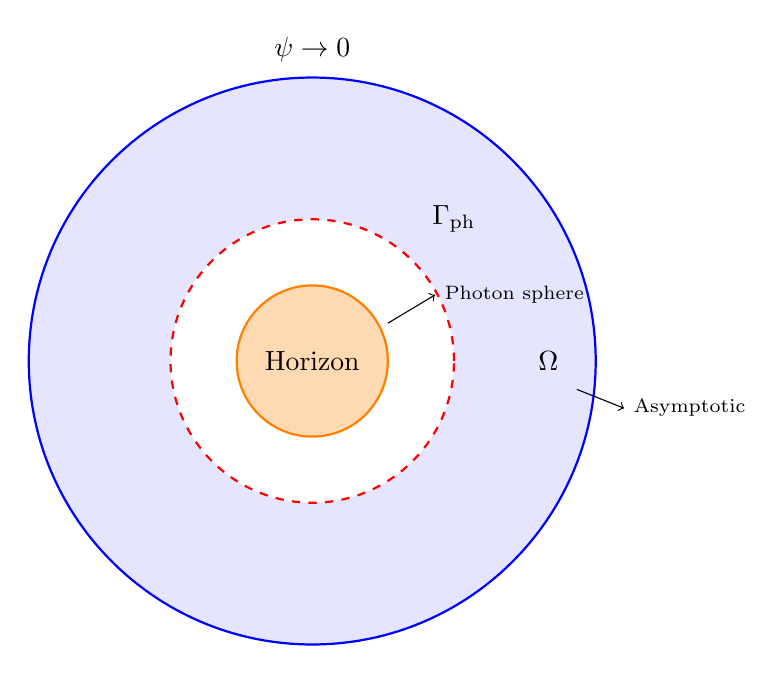
\begin{tikzpicture}[scale=1.2]
% Exterior region
\fill[blue!10] (0,0) circle (3);
\fill[white] (0,0) circle (1.5);
\fill[orange!30] (0,0) circle (0.8);
% Boundaries
\draw[thick, blue] (0,0) circle (3);
\draw[thick, red, dashed] (0,0) circle (1.5);
\draw[thick, orange] (0,0) circle (0.8);
% Labels
\node at (0,0) {Horizon};
\node at (1.5, 1.5) {$\Gamma_{\rm ph}$};
\node at (2.5, 0) {$\Omega$};
\node at (0, 3.3) {$\psi \to 0$};
% Annotations
\draw[->] (0.8, 0.4) -- (1.3, 0.7);
\node[right] at (1.3, 0.7) {\scriptsize Photon sphere};
\draw[->] (2.8, -0.3) -- (3.3, -0.5);
\node[right] at (3.3, -0.5) {\scriptsize Asymptotic};
\end{tikzpicture}
\caption{Domain structure for exterior problems. The solution domain 
$\Omega$ (blue) excludes the optical horizon region (orange). The photon 
sphere $\Gamma_{\rm ph}$ (red dashed) carries a nonlinear Robin condition.
Asymptotic flatness is imposed at infinity.}
\label{fig:exterior_domain}
\end{figure}

\begin{theorem}[Exterior well-posedness]\label{thm:exterior}
Under assumptions (A1)--(A4) and the boundary conditions above, there 
exists a weak solution $\psi \in W^{1,p}_{\rm loc}(\Omega)$ with the 
correct decay at infinity. If the boundary operators are strictly monotone, 
the solution is unique.
\end{theorem}

The proof extends standard techniques by using weighted Sobolev spaces 
to handle the unbounded domain.

%-----------------------------------------------------------------------------
% §3.3 DYNAMIC/HYPERBOLIC CASE
%-----------------------------------------------------------------------------
\subsection{Dynamic Solutions: Hyperbolic Theory}\label{sec:hyperbolic}

For time-dependent problems, the field equation becomes:
\begin{equation}
\frac{1}{c^2}\partial_t^2\psi - \nabla\cdot[\mufunction(|\nabla\psi|/\astar)\nabla\psi] 
= -\frac{8\pi G}{c^2}(\rho - \bar{\rho}).
\label{eq:dynamic_field}
\end{equation}
This is a quasilinear wave equation with nonlinear principal part.

\subsubsection{First-Order Symmetric Hyperbolic Form}

Equation~\eqref{eq:dynamic_field} can be rewritten as a first-order 
symmetric hyperbolic system. Introduce:
\begin{equation}
U = (\psi, \partial_t\psi, \partial_1\psi, \partial_2\psi, \partial_3\psi)^T.
\end{equation}
The evolution takes the form:
\begin{equation}
\partial_t U + A^i(U)\partial_i U = S(U, \mathbf{x}),
\label{eq:first_order_system}
\end{equation}
where $A^i(U)$ are symmetric matrices depending on the state $U$, and 
$S$ contains source terms.

Hyperbolicity requires the matrices $A^i$ to satisfy:
\begin{equation}
\det\!\left(\sum_i n_i A^i\right) \neq 0 \quad \forall\,\mathbf{n} \neq 0.
\end{equation}
This is equivalent to the condition $\mufunction'(x) > 0$---the same 
monotonicity condition (A4) ensuring ellipticity in the static case.

\subsubsection{Local Well-Posedness}

\begin{theorem}[Local existence]\label{thm:local_cauchy}
Let initial data $(\psi_0, \psi_1) \in H^s(\mathbb{R}^3) \times H^{s-1}(\mathbb{R}^3)$ 
with $s > 5/2$. Under assumptions (A1)--(A4), there exists $T > 0$ and a 
unique solution
\begin{equation}
\psi \in C([0,T]; H^s) \cap C^1([0,T]; H^{s-1})
\end{equation}
of the Cauchy problem for~\eqref{eq:dynamic_field}.
\end{theorem}

The proof uses standard symmetric-hyperbolic theory: energy estimates 
control $H^s$ norms, and iteration in time extends the local solution.

\paragraph{Limitation: Global existence.}
Global existence (arbitrary long times) is not guaranteed. The main 
obstruction is potential gradient blow-up in finite time, analogous to 
shock formation in nonlinear wave equations.

For physically realistic sources (slowly evolving matter distributions), 
solutions exist on timescales $T \gg c/a_0 \sim H_0^{-1}$---far 
longer than any astrophysical process. Numerical evidence suggests smooth 
solutions persist for all astrophysically relevant scenarios.

\subsubsection{Finite Speed of Propagation}

\begin{theorem}[Causality]\label{thm:causality}
Solutions of~\eqref{eq:dynamic_field} satisfy:
\begin{enumerate}
\item All characteristic speeds are $\leq c$.
\item The domain of dependence of a point $(t, \mathbf{x})$ is contained 
in the backward light cone $\{(t', \mathbf{x}'): |\mathbf{x} - \mathbf{x}'| 
\leq c(t - t')\}$.
\item No signal propagates faster than $c$.
\end{enumerate}
\end{theorem}

This follows from the structure of the characteristic matrix 
$\sum_i n_i A^i$: its eigenvalues (characteristic speeds) are bounded 
by $c$ under the convexity conditions on $\Wfunc$.

Causality is a crucial physical requirement. \DFD satisfies it by 
construction: the TT sector propagates at exactly $c$, and the scalar 
sector propagates at speeds $\leq c$ for all admissible $\mufunction$.

%-----------------------------------------------------------------------------
% §3.4 STABILITY
%-----------------------------------------------------------------------------
\subsection{Stability}\label{sec:stability}

\subsubsection{Energy Positivity}

\begin{theorem}[Positive energy]\label{thm:positive_energy}
If $\Wfunc$ is strictly convex, then:
\begin{enumerate}
\item The energy functional $\mathcal{E}[\psi] \geq 0$ for all 
$\psi$ satisfying asymptotic flatness.
\item Static solutions are local energy minima.
\item There are no negative-energy (ghost) modes in the linearized theory.
\end{enumerate}
\end{theorem}

\paragraph{Proof sketch.}
Convexity of $\Wfunc$ implies convexity of the energy density $H(\xi)$. 
The integral $\mathcal{E}[\psi]$ inherits this convexity. For 
asymptotically flat configurations, $\mathcal{E}[\psi = 0] = 0$ (vacuum), 
and convexity ensures all other configurations have $\mathcal{E} \geq 0$.

\subsubsection{Perturbative Stability}

Consider small perturbations $\delta\psi$ about a static solution $\psi_0$:
\begin{equation}
\psi = \psi_0 + \delta\psi, \quad |\delta\psi| \ll |\psi_0|.
\end{equation}
The linearized equation for $\delta\psi$ is:
\begin{equation}
\frac{1}{c^2}\partial_t^2(\delta\psi) - \nabla\cdot[M_{ij}(\nabla\psi_0)
\nabla_j(\delta\psi)] = 0,
\end{equation}
where the effective mass matrix is:
\begin{equation}
M_{ij} = \mufunction(x_0)\delta_{ij} + \mufunction'(x_0)\frac{(\partial_i\psi_0)
(\partial_j\psi_0)}{|\nabla\psi_0|\,\astar},
\end{equation}
with $x_0 = |\nabla\psi_0|/\astar$. The denominator $|\nabla\psi_0|\,\astar$ ensures dimensional consistency: since $[(\partial_i\psi_0)(\partial_j\psi_0)] = \text{m}^{-2}$ and $[|\nabla\psi_0|\,\astar] = \text{m}^{-2}$, the ratio is dimensionless.

Under conditions (A4), $M_{ij}$ is positive definite. The linearized 
operator has only real, positive eigenfrequencies---no growing modes, 
no instabilities.

\subsubsection{No Ghosts}

A ghost is a degree of freedom with wrong-sign kinetic term, leading to 
negative-energy states. In \DFD:
\begin{itemize}
\item The scalar $\psi$ has kinetic term $\propto \Wfunc'(X) > 0$ by (A4).
\item The TT modes $h_{ij}^{\rm TT}$ have standard positive kinetic term 
from~\eqref{eq:action_gw}.
\end{itemize}
Total degrees of freedom: $1 + 2 = 3$, all with positive kinetic energy. 
No ghosts.

%-----------------------------------------------------------------------------
% §3.5 INITIAL-BOUNDARY VALUE PROBLEMS
%-----------------------------------------------------------------------------
\subsection{Initial-Boundary Value Problems}\label{sec:ibvp}

For laboratory experiments and numerical simulations in finite volumes, 
we require well-posedness of the initial-boundary value problem (IBVP). 
This is the natural setting for terrestrial tests of \DFD.

\subsubsection{Dynamic Structural Assumptions}

The dynamic field equation can be written in the general quasilinear form:
\begin{equation}
a^{\mu\nu}(\psi,\partial\psi)\partial_\mu\partial_\nu\psi 
+ b^\mu(\psi,\partial\psi,x)\partial_\mu\psi + c(\psi,\partial\psi,x) = S(x),
\label{eq:dynamic-general}
\end{equation}
where $a^{\mu\nu}$ forms the principal symbol and $b^\mu$, $c$ are lower-order 
terms. Well-posedness requires:

\begin{itemize}
\item[\textbf{(A1$'$)}] \textbf{Uniform hyperbolicity:} There exists $\lambda \geq 1$ 
such that $a^{\mu\nu}\xi_\mu\xi_\nu$ has Lorentzian signature compatible with 
$\eta^{\mu\nu}$. For timelike covectors ($\eta^{\mu\nu}\xi_\mu\xi_\nu < 0$), 
$a^{\mu\nu}\xi_\mu\xi_\nu < 0$; for spacelike covectors,
\begin{equation}
\lambda^{-1}\eta^{\mu\nu}\xi_\mu\xi_\nu \leq a^{\mu\nu}\xi_\mu\xi_\nu \leq \lambda\eta^{\mu\nu}\xi_\mu\xi_\nu.
\end{equation}

\item[\textbf{(A2$'$)}] \textbf{Lower-order regularity:} For $|\alpha| \leq s$ 
(with $s > 5/2$), the derivatives $\partial^\alpha b^\mu$, $\partial^\alpha c$ 
are continuous and polynomially bounded in $|\psi|$, $|\partial\psi|$.

\item[\textbf{(A3$'$)}] \textbf{Source regularity:} $S(x) \in H^{s-1}$ on the 
spatial domain.
\end{itemize}

These are satisfied by the \DFD strong-field equation whenever $\psi$ and 
$\partial\psi$ remain bounded.

\subsubsection{IBVP Formulation}

Let $\Omega \subset \mathbb{R}^3$ be bounded with smooth boundary 
$\partial\Omega$. The Dirichlet IBVP is:
\begin{equation}
\begin{cases}
a^{\mu\nu}(\psi,\partial\psi)\partial_\mu\partial_\nu\psi + \text{l.o.t.} = S(x), 
& (t,\mathbf{x}) \in [0,T] \times \Omega \\
\psi(0,\mathbf{x}) = \psi_0(\mathbf{x}), & \mathbf{x} \in \Omega \\
\partial_t\psi(0,\mathbf{x}) = \psi_1(\mathbf{x}), & \mathbf{x} \in \Omega \\
\psi(t,\mathbf{x}) = g(t,\mathbf{x}), & (t,\mathbf{x}) \in [0,T] \times \partial\Omega
\end{cases}
\label{eq:ibvp-formulation}
\end{equation}

\subsubsection{Compatibility Conditions}

Regularity requires the initial and boundary data to be compatible at 
$\{t = 0\} \cap \partial\Omega$:
\begin{itemize}
\item \textbf{Zeroth order:} $\psi_0|_{\partial\Omega} = g(\cdot,0)$
\item \textbf{First order:} $\psi_1|_{\partial\Omega} = \partial_t g(\cdot,0)$
\item \textbf{$k$-th order:} $\partial_t^k\psi|_{t=0,\partial\Omega} = \partial_t^k g(\cdot,0)$
\end{itemize}
For solutions in $H^s(\Omega)$ with $s > 5/2$, compatibility is required up 
to order $\lfloor s - 1 \rfloor$.

\subsubsection{Energy Estimates}

Define the Sobolev energy:
\begin{equation}
E_s(t) = \sum_{|\alpha| \leq s} \int_\Omega \big(|\partial^\alpha\partial_t\psi|^2 
+ |\nabla\partial^\alpha\psi|^2\big)\,d^3x.
\label{eq:sobolev-energy}
\end{equation}

Under assumptions (A1$'$)--(A3$'$) with compatibility conditions:
\begin{equation}
\frac{d}{dt}E_s(t) \leq C(M)\big(E_s(t) + \|S\|^2_{H^{s-1}(\Omega)} 
+ \|g\|^2_{H^{s-1/2}(\partial\Omega)}\big),
\label{eq:energy-differential}
\end{equation}
where $C(M)$ depends on bounds for $\psi$, $\partial\psi$ in $L^\infty$.

By Gronwall's lemma:
\begin{equation}
\resizebox{0.9\columnwidth}{!}{$\displaystyle
\boxed{
E_s(t) \leq e^{C(M)t}\Big(E_s(0) + \int_0^t \big(\|S\|^2_{H^{s-1}} + \|g\|^2_{H^{s-1/2}}\big)\,d\tau\Big)
}
$}
\label{eq:gronwall-bound}
\end{equation}

This establishes continuous dependence on initial and boundary data.

\subsubsection{Main IBVP Theorem}

\begin{theorem}[IBVP Well-Posedness]\label{thm:ibvp}
Let $\Omega \subset \mathbb{R}^3$ be bounded with smooth boundary and 
$s > 5/2$. Under assumptions (A1$'$)--(A3$'$), given:
\begin{itemize}
\item Initial data $(\psi_0, \psi_1) \in H^s(\Omega) \times H^{s-1}(\Omega)$
\item Source $S \in H^{s-1}(\Omega)$
\item Boundary data $g \in H^s([0,T] \times \partial\Omega)$
\item Compatibility conditions up to order $\lfloor s - 1 \rfloor$
\end{itemize}
there exists $T > 0$ and a unique solution
\begin{equation}
\psi \in C^0([0,T]; H^s(\Omega)) \cap C^1([0,T]; H^{s-1}(\Omega))
\end{equation}
depending continuously on $(\psi_0, \psi_1, S, g)$ in the natural Sobolev norms.
\end{theorem}

\paragraph{Proof sketch.}
The proof uses standard techniques for quasilinear hyperbolic IBVP. 
Linearization around an approximate solution, energy estimates with 
boundary multipliers, and Picard iteration in a suitable Banach space 
yield existence and uniqueness. The compatibility conditions control 
boundary terms in the energy estimates.

\subsubsection{Finite Speed of Propagation}

\begin{theorem}[Finite Speed]\label{thm:finite-speed}
Let $\psi$ and $\tilde\psi$ be solutions of~\eqref{eq:dynamic_field} with 
initial data coinciding in a ball $B_R(\mathbf{x}_0)$. There exists a 
characteristic speed $c_{\rm char} > 0$ (depending only on the hyperbolicity 
constant $\lambda$) such that
\begin{equation}
\psi(t,\mathbf{x}) = \tilde\psi(t,\mathbf{x}) \quad \text{for } 
|\mathbf{x} - \mathbf{x}_0| \leq R - c_{\rm char}t.
\end{equation}
\end{theorem}

This ensures causality: disturbances propagate at finite speed bounded by $c$.

\subsubsection{Parabolic Extension}

For dissipative problems or numerical relaxation schemes, the parabolic 
extension is relevant:
\begin{equation}
\partial_t\psi - \nabla\cdot[\mufunction(|\nabla\psi|)\nabla\psi] = f(t,\mathbf{x}).
\label{eq:parabolic-extension}
\end{equation}

\begin{theorem}[Parabolic Well-Posedness]\label{thm:parabolic}
Under assumptions (A1)--(A4), there exists a unique evolution
\begin{equation}
\psi \in L^p(0,T; W^{1,p}(\Omega)) \cap C([0,T]; L^2(\Omega)).
\end{equation}
If $f$ is time-independent and boundary operators are dissipative, 
solutions converge to a steady state as $t \to \infty$.
\end{theorem}

This follows from Crandall--Liggett theory: the monotone operator 
$A\psi = -\nabla\cdot\mathbf{a}(\nabla\psi)$ generates a contraction 
semigroup on $L^2(\Omega)$.

\subsubsection{Stability Estimates}

\begin{theorem}[Continuous Dependence]\label{thm:continuous-dependence}
Let $\psi_1$, $\psi_2$ be solutions with data $(f_1, BC_1)$, $(f_2, BC_2)$ 
respectively. If $\mathbf{a}$ is strongly monotone and locally Lipschitz:
\begin{equation}
\|\nabla(\psi_1 - \psi_2)\|_{L^p(\Omega)} \leq C\big(\|f_1 - f_2\|_{V'} 
+ \|BC_1 - BC_2\|_{\partial\Omega}\big).
\end{equation}
\end{theorem}

This ensures physical stability: small changes in sources or boundary 
conditions produce small changes in solutions.

\subsubsection{Numerical Implementation}

The weak form~\eqref{eq:weak_form} is directly implementable in finite 
element packages. The Newton iteration Jacobian is:
\begin{equation}
A_{ij}(\nabla\psi) = \mufunction(|\nabla\psi|)\delta_{ij} 
+ \mufunction'(|\nabla\psi|)\frac{\partial_i\psi\,\partial_j\psi}{|\nabla\psi|}.
\label{eq:fem-jacobian}
\end{equation}

\paragraph{Regularization.}
At $|\nabla\psi| \to 0$, the Jacobian may become ill-conditioned. A practical 
remedy is to replace $|\nabla\psi|$ by $\sqrt{|\nabla\psi|^2 + s_0^2}$ with 
small $s_0 > 0$.

%-----------------------------------------------------------------------------
% §3.6 OPEN MATHEMATICAL PROBLEMS
%-----------------------------------------------------------------------------
\subsection{Open Mathematical Problems}\label{sec:math_open}

Several mathematical questions remain open:

\begin{enumerate}
\item \textbf{Global existence for dynamic equations:} Does the Cauchy 
problem have global-in-time solutions for generic initial data? Shock 
formation cannot be ruled out mathematically, though physical arguments 
suggest smoothness persists.

\item \textbf{Uniqueness with horizon boundary:} The one-way horizon 
boundary condition (ingoing flux only) is physically motivated but 
mathematically nonstandard. A rigorous uniqueness theorem for this 
asymmetric condition is not yet established.

\item \textbf{Horizon regularity:} Near optical horizons, the nonlinear 
boundary conditions may require specialized function spaces. Regularity 
results near horizons with asymmetric BCs remain open.

\item \textbf{Strong-field numerical convergence:} Finite element 
implementations work well in the weak-field regime, but convergence 
rates near optical horizons require further study.

\item \textbf{Gradient blow-up and singularity formation:} Can solutions 
develop gradient singularities (analogous to shock formation) in finite 
time? Physical scenarios suggest not, but mathematical proof is lacking.

\item \textbf{Coupling to quantum fields:} The semi-classical regime 
(quantum matter on classical $\psi$ background) is well-defined. Full 
quantization of $\psi$ is unnecessary: the action scales as $S_\psi \sim (M_P/a_\star)^2 \gg \hbar$, 
ensuring quantum fluctuations are negligible. The gauge emergence framework 
provides the connection to particle physics (\S\ref{sec:quantum}).
\end{enumerate}

These technical open problems do not affect the physical predictions in 
\S\ref{sec:ppn}--\S\ref{sec:matter_wave}, which operate in well-understood 
weak-field or linearized regimes.

%-----------------------------------------------------------------------------
% §3 SUMMARY
%-----------------------------------------------------------------------------
\subsection{Summary of Section~\ref{sec:wellposed}}

The \DFD field equations are mathematically well-posed:

\begin{table}[h]
\caption{Well-posedness summary.}
\label{tab:wellposed_summary}
\begin{ruledtabular}
\scriptsize
\begin{tabular}{lccc}
Property & Static & Dyn. & IBVP \\
\hline
Existence & \checkmark & \checkmark (loc.) & \checkmark (loc.) \\
Uniqueness & \checkmark (str.\ mon.) & \checkmark (loc.) & \checkmark (compat.) \\
Regularity & $C^{1,\alpha}_{\rm loc}$ & $H^s$ pres. & $H^s$ pres. \\
Stability & \checkmark (convex $\Wfunc$) & \checkmark & \checkmark (Gron.) \\
Causality & --- & $c_{\rm char} \leq c$ & $c_{\rm char} \leq c$ \\
No ghosts & \checkmark & \checkmark & \checkmark \\
\end{tabular}
\end{ruledtabular}
\end{table}

The mathematical foundations are solid: existence and uniqueness theorems, 
regularity results, stability guarantees, causal propagation, and explicit 
energy estimates. The IBVP formulation enables rigorous treatment of 
laboratory-scale experiments in bounded domains. This places \DFD on equal 
footing with \GR as a mathematically consistent classical field theory.
